\subsection{Measured application and its cost limit}
We use six positive-kernel families at $n=256,1024,2048$: a positive
lognormal matrix, two line Gaussian kernels, and three plane Gaussian
kernels. Line marginals shift with the seed; plane supports and masses
are sampled independently. Settings were screened on seed zero and held
fixed for seeds one and two. Five repetitions per method and problem
are shuffled after warm-up on the M4 CPU with single-thread BLAS.
The output phase normalizes rows exactly and stops at
$\max_j|c_j/b_j-1|\leq10^{-9}$. Common input-kernel construction is
excluded; all method-specific setup, unsuccessful work, checks, and
scaling-factor reconstruction are included. Dense plan materialization
is excluded for every method.
All 720 general solves and 120 structured solves reach the target.
This is matched marginal accuracy, not a certified objective-gap comparison.

\begin{table}[!hbp]\centering\small
\begin{tabular}{lrrrr}\toprule
Problem & Ordinary & Frozen 4 & Changing 4 & Changing 2\\\midrule
Line, $\varepsilon=0.02$ & 85.66 & 62.29 & 80.11 & 80.22\\
Line, $\varepsilon=0.003$ & 547.80 & 349.35 & 493.13 & 426.58\\
Plane, $\varepsilon=0.03$ & 57.37 & 49.11 & 58.56 & 61.41\\
Plane, $\varepsilon=0.006$ & 281.61 & 191.12 & 276.25 & 243.55\\
Plane, $\varepsilon=0.003$ & 564.03 & 380.82 & 536.28 & 459.07\\
\bottomrule\end{tabular}
\caption{Complete solve times in milliseconds at $n=2048$, reported as
the median of per-seed five-repeat medians. The matched four-direction
comparison isolates the added changing-rule model; the two-direction
version also changes representation capacity.}\label{tab:entropic-cost}
\end{table}


The two-direction changing-rule model is $1.13$--$1.33\times$ faster
than ordinary iteration on the three narrow-kernel cases at $n=1024$,
and $1.16$--$1.28\times$ at $n=2048$. It loses on every nontrivial
$n=256$ case. At $n=2048$ the frozen control is faster than either
changing-rule variant on all five nontrivial cases. The positive
lognormal control finishes before acquisition begins; its timing
differences are noise. These controls do not establish superiority over
Anderson, overrelaxed Sinkhorn, continuation, or specialized OT solvers.

\begin{figure}[tb]\centering
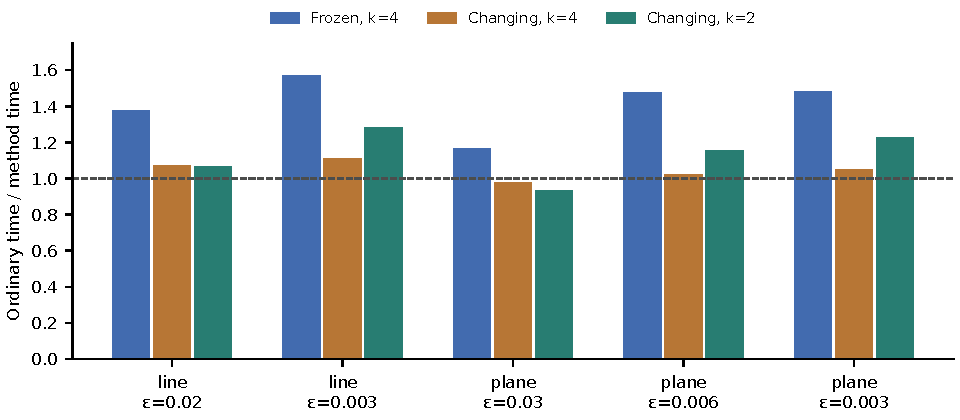
\includegraphics[width=\linewidth]{figures/entropic_cost.pdf}
\caption{General-kernel speedups at $n=2048$. Values above one are faster
than ordinary iteration. Ratios are summarized within seed before
aggregation. Better modeling of the evolving rule does not yet offset
its acquisition cost relative to the frozen control.}\label{fig:entropic-cost}
\end{figure}

For the narrow-line case, median actual map evaluations are 198,186,193
for frozen four, changing four, and changing two, respectively. Their
kernel-vector products are 648,1114,686. Batched products need not have
the same per-vector cost, but these counts explain why fewer full passes
are insufficient evidence of a faster method.

An independent diagnostic holds the four-direction basis fixed and
compares horizons 16 and 32 at ordinary prefixes 8,32,128, for size 128
and seeds zero and one. Already-converged anchors are skipped.
Of 52 paired comparisons, the quadratic model improves state prediction
in 39 and the projected endpoint-derivative prediction in 36. Fifty
pairs complete for both models; two unrestricted quadratic rollouts do
not complete. No evaluated finite-trajectory bound is violated. True
future states are used only for this untimed diagnostic, never by the solver.

\begin{figure}[tb]\centering
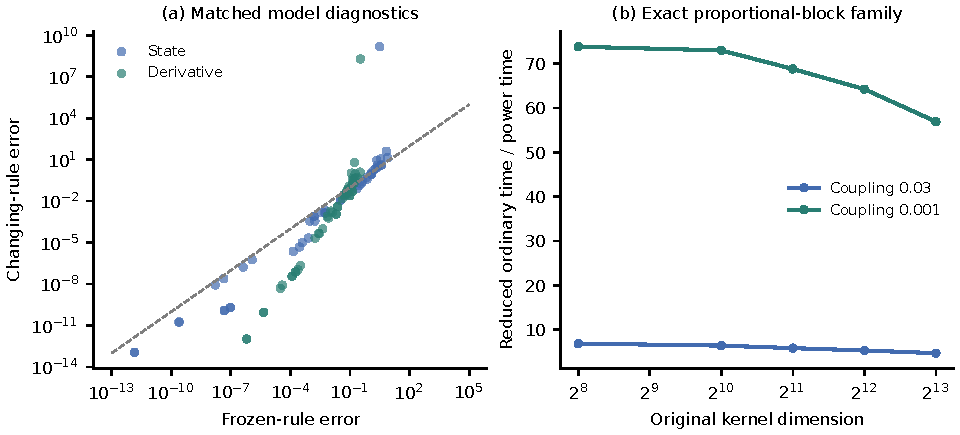
\includegraphics[width=\linewidth]{figures/entropic_closure.pdf}
\caption{(a) All 50 completed pairs in the unrestricted matched-model
diagnostic; below the diagonal favors the changing rule. Two additional
quadratic rollouts fail to complete. Derivative errors concern the same
anchor-projected operator, not a full operator-norm certificate.
(b) Exact projective-power speedups over ordinary iteration using the
same supplied block reduction, including full scaling-factor readout.}
\label{fig:entropic-closure}\end{figure}

For the exact two-group family, both comparators use
\eqref{eq:sinkhorn-block-map}. The power method increases its finite
horizon geometrically and checks the actual reduced marginal residual.
Across original dimensions 256 through 8192, the speedup is
$4.7$--$6.9\times$ for block coupling $.03$ and
$56.9$--$73.8\times$ for coupling $.001$. The latter reduced ordinary
runs take approximately 14--15 ms, versus $.19$--$.26$ ms for powers
and reconstruction. This family validates economical exact closure;
it does not demonstrate discovery of that structure on arbitrary kernels.

A separate earlier transfer study, retained with the source, compared
fixed polynomial, discovery, and Anderson methods on 24 image-mass and
Gaussian-mixture problems. It used a different marginal norm, checking
cadence, sizes, and acquisition policy. Its timings are not pooled here.
Anderson was generally stronger there; the present experiment isolates
the cost of carrying the evolving rule rather than establishing a new
best general Sinkhorn solver.
